\documentclass{article}
\usepackage[utf8]{inputenc}
\usepackage{amsmath}
\usepackage{listings}
\usepackage{geometry}
\usepackage{graphicx}
\usepackage{subfig}
\usepackage[colorlinks=true]{hyperref}
\title{%
Project 1 - Regression, Resampling and Data analysis\\
\large FYS-STK3155 at University of Oslo}
\author{Simen Løken}
\date{October 2020}
\footskip = 90pt
\topmargin = -40pt
\begin{document}
\nocite{proj1}
\maketitle
\section{Abstract}
In this project we'll discuss and analyze three different regression methods and two different examples of resampling. We do this so as to show how one can assess the different methods and how to consider which one is best suited for your particular purpose. \newline
We find that for all methods, variables can be a tricky thing, and we have to be careful when picking 'free varaibles' such as our data points N or our parameters for bootstrap runs or Cross-Validation folds.
\section{Introduction}
At the heart of machine learning lies a few important statistical methods, namely regression and \newline resampling. Regression is the method of comparing an dependent response variable to another (or several) independent variable(s) and examine their relationship(s). In it's most general form, for some set of variables $\mathbf{X}$, and a dependent variable $y$, it'd take the form:
\begin{equation} \label{1}
    y = \beta_0 + \beta_1 \mathbf{X} + \epsilon
\end{equation}
\newline where $\epsilon$ is the error
\newline with possibility for expansion given multiple variables $\mathbf{X}$ as:
\begin{equation*}
    y = \beta_0 + \beta_1 \mathbf{X}_1 + \beta_2 \mathbf{X}_2 \cdots \beta_{n-1} \mathbf{X}_{n-1} + \beta_n \mathbf{X}_n + \epsilon
\end{equation*}
\newline
This is where resampling comes in. If we can seperate our dataset $\mathbf{X}$ into subsets, and use one of our subsets to better fit our dependent variable $y$, we can then use the remaining independent subsets to best possibly fit our data. \newline
In this report we're going to be looking at two statistical methods for resampling, bootstrapping and cross-validation. We're going to be employing three regression analysis methods with each of these, OLS (Ordinary Least Squares), LASSO (Least Absolute Shrinkage and Selection Operator) and Ridge regression.
We're going to employ these methods onto two seperate datasets, one we create on our own using the Franke Function, and one supplied by UiO containing geographical data of an area close to Stavanger, Norway.
\section{Theory and Method}
Like previously mentioned, we're going to be employing the Franke Function, which is defined as:
\begin{align*}
f(x,y) &= \frac{3}{4}\exp{\left(-\frac{(9x-2)^2}{4} - \frac{(9y-2)^2}{4}\right)}+\frac{3}{4}\exp{\left(-\frac{(9x+1)^2}{49}- \frac{(9y+1)}{10}\right)} \\
&+\frac{1}{2}\exp{\left(-\frac{(9x-7)^2}{4} - \frac{(9y-3)^2}{4}\right)} -\frac{1}{5}\exp{\left(-(9x-4)^2 - (9y-7)^2\right)} 
\end{align*}
\newline
This will allow us, for a randomly generated array $x$ and $y$, to create a dataset spanning the dimensions of the array $x$ and $y$, in addition to letting us create a design matrix, henceforth referred to as $\mathbf{X}$. We're defining $\mathbf{X}$ to be:
\begin{equation*} \mathbf{X} = 
    \begin{bmatrix} 1& x_1^1& y_1^1& x_1^1y_1^1& \cdots& x_1^oy_1^o \\
    1 & x_2^1& y_2^1& x_2^1y_2^1& \cdots& x_2^oy_2^o \\
    \vdots& \vdots& \vdots& \vdots& \vdots& \vdots \\
    1& x_n^1& y_n^1& x_n^1y_n^1& \cdots& x_n^oy_n^o
    \end{bmatrix} 
                                 
\label{eq:matrixse} 
\end{equation*}
\newline
where $o$ is the order of our polynomial, in other words, it's complexity. Knowing this, let's take a look at the methods we're going to be using.
\subsection{OLS}
Given what we know from Equation [\ref{1}], then an approximation of y $\Tilde{y}$ can be expressed as:
\begin{equation}
    \Tilde{y} = \mathbf{X}\beta
\end{equation}
We can then define a function over which measures the spread of values $y_i$ and the parameterized $\Tilde{y}$.
\begin{equation*}
    C(\beta) = \frac{1}{n} \left ((y-\mathbf{X}\beta)^T (y-\mathbf{X}\beta) \right)
\end{equation*}
which can be simplified as:
\begin{equation}
    C(\beta)=\frac{1}{n} \sum_{i=0}^{n-1} (y_i - \Tilde{y}_i)^2
\end{equation}
Additionally, we have
\begin{equation}
    \frac{\delta C(\beta)}{\delta \beta} = 0 = \mathbf{X}^T (y-\mathbf{X}\beta)
\end{equation}
which then means:
\begin{equation} \label{2}
    \beta = \frac{\mathbf{X}^Ty}{\mathbf{X}^T\mathbf{X}}
\end{equation}
We can then use these values to perform our OLS operation.
If we find $\beta$ through Equation [\ref{2}], then we can use that to find $\Tilde{y}$ and it's accompanying predictor-array through the python code:
\begin{lstlisting}[language=Python]
    B = np.linalg.inv(X_train.T @ X_train) @ X_train.T @ y_train
    ytilde = X_train @ B
    ypred = X_test  @ B
\end{lstlisting} \newline
which can then be used to finishing with one of our resampling methods.
\subsection{Ridge Regression}
We modify our existing equation to include such that:
\begin{equation*}
    \mathbf{X}^T\mathbf{X}\xrightarrow[]{}\mathbf{X}^T\mathbf{X}+\lambda I
\end{equation*}
As such we modify our other existing equations and get
\begin{equation} \label{3}
    \beta_{Ridge} = \frac{\mathbf{X}^Ty+\lambda I}{\mathbf{X}^Ty}
\end{equation}
Our new variables, $I$ and $\lambda$ are the identity matrix and a parameter, respectively. $\lambda$ is a parameter that represents the amount of shrinkage in the coefficients $\beta$.
\subsection{LASSO Regression}
LASSO is very similar in form to the Ridge Regression, but it instead yields nonlinear solutions and as such has no closed form expression.
We express $\beta$ as:
\begin{equation*}
    \beta = argmin \sum_{i=1}^{N} \left (y_i - \beta_0 - \sum_{j+1}^{p}x_{ij}\beta_{j} \right)^2
\end{equation*}
\newline
restricted by 
\begin{equation*}
    \sum_{j=1}^{p}|\beta_j| \leq t
\end{equation*}
which is practically identical to the non-vector form of Equation [\ref{3}], the only difference being that Equation [\ref{3}] is resticted by
\begin{equation*}
    \sum_{j=1}^{p}\beta_j^2 \leq t
\end{equation*}
\newpage
\subsection{Resampling}
\subsubsection{Bootstrap}
The bootstrap method perhaps the most 'basic' of the resampling methods we're going to be using. In a short, non-code, we're looking to:
\begin{itemize}
    \item Draw numbers for observed variables (training data, in our case), replace afterwards
    \item Create an array with the drawn values
    \item Apply these drawn values onto our model
    \item Return the mean of our calculations
    \item repeat for N-times
    \item This is done for each polynomial order, going from 0 up to some polynomial degree $o$
\end{itemize}
When we're done with this, we can use our predictive values and retrieve the Mean-Squared-Error of our method for each given polynomial order $o$
\subsubsection{Cross Validation}
Cross-validation is, in theory, a bit more "stable" and perhaps more useful than the bootstrap method. \newline
In short, we're looking to
\begin{itemize}
    \item Shuffle dataset
    \item Split dataset into $k$ groups
\end{itemize}
For each unique group:
\begin{itemize}
    \item Dedicate a group as test data
    \item Use remaining groups as training data
    \item Fit training data onto a selected model(OLS, LASSO etc..), evaluate this onto the test data
    \item Discard model, retain evaluation score.

\end{itemize}
After doing this we can extract from our evaluation score the Mean-Squared-Error of our method using shrinkage parameters $\lambda$
\subsection{Estimating Errors}
We've talked a fair bit about the Mean-Squared-Error, but we've yet to see what it actually looks like. As given by our assignment [\cite{oppgtxt}], MSE is defined as:
\begin{equation*}
    MSE(\hat{y},\hat{\tilde{y}}) = \frac{1}{n}
\sum_{i=0}^{n-1}(y_i-\tilde{y}_i)^2
\end{equation*}
\newline and the R2 score is defined as:
\begin{equation*}
    R^2(\hat{y}, \tilde{\hat{y}}) = 1 - \frac{\sum_{i=0}^{n - 1} (y_i - \tilde{y}_i)^2}{\sum_{i=0}^{n - 1} (y_i - \bar{y})^2}
\end{equation*}
\newline
These both have in common that they tell you something about how good a fit is in relation to it's actual analytical value. MSE (obviously) tells you the mean-squared error of your fit, or rather. We can then use this in addendum with a regression and resampling model, to best find out which is the best fit for our particular situation. We can also use MSE to find out which polynomial order is the best fit for our situation. If we calculate MSE for each polynomial order, then the one with the lowest value should in theory be the best fit for our particular situation, atleast within area we are checking.
\newline
The R2 score measures how much of our variance in our dependent variable is explained by an independent variable. So let's say we have and R2 of .99: That means that .99 of our observed variations can be explain by our model. That means that the closer we are to 1, the better.
\section{Results}
Firstly, a three-dimensional plot of the Franke Function over a meshgrid is:
\begin{figure}[ht!]
    \centering
    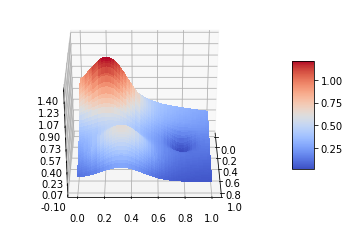
\includegraphics[scale=0.8]{figure1.png}
    \caption{A standard, analytical solution to the Franke Function over a two dimensional meshgrid.}
    \label{fig:my_label}
\end{figure}
\newline
Now let's look at a statistical solution using the OLS method, using different polynomial orders to see which is a better fit.
\begin{figure}
\centering
\subfloat[Polynomial order: 2]{
  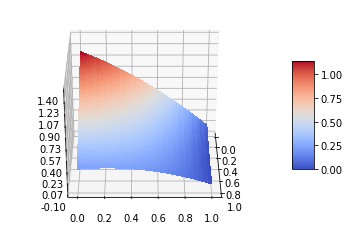
\includegraphics[width=65mm]{figure2.png}
}
\subfloat[Polynomial order: 4]{
  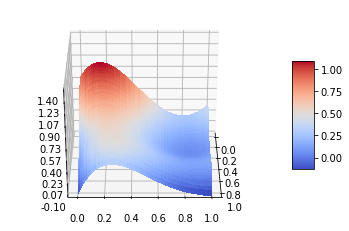
\includegraphics[width=65mm]{figure3.png}
}
\newline
\subfloat[Polynomial order: 7]{
  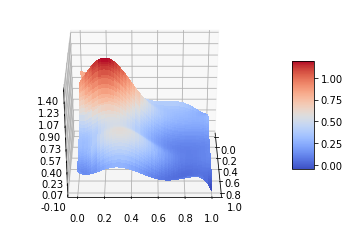
\includegraphics[width=65mm]{figure4.png}
}
\subfloat[Polynomial order: 20]{
  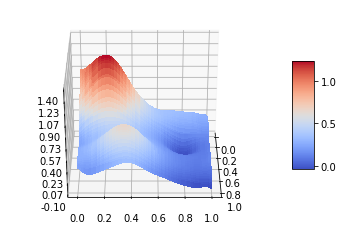
\includegraphics[width=65mm]{figure5.png}
}
\newline
\subfloat[Polynomial order: 27]{
  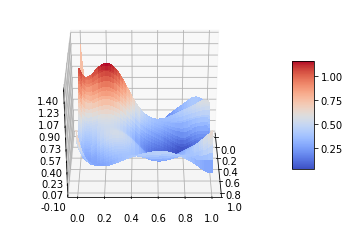
\includegraphics[width=65mm]{figure6.png}
}
\caption{Here are five different statistical solutions using OLS to plot the Franke Function. Notice how as we approach a break-point for the best possible fit (7 in a set with these values) it starts to look more and more like the analytical solution shown in figure [\ref{fig:my_label}]. Once we're past that point, we move into overfitting. Notice how for (e) it's features are greatly exaggerated. \newline These are all without noise, naturally.}
\end{figure}
Now let's look at some data given by our OLS-fit for the polynomial order 7:
\newpage We find, using our error estimates:
\begin{table}[ht!]
    \centering
    \begin{tabular}{c|c|c}
        & Training& Testing&  \\
        MSE & 0.15340805& 0.15295584& \\
        R2 & -0.99540759& -0.99210637
    \end{tabular}
    \caption{Error estimates and R2 scores for polynomial order = 7 \newline
    I can't explain why R2 is negative. Maybe I was supposed to square it?}
    \label{tab:my_label}
\end{table}
\newline
Let's now examine the Bias-variance trade-off. We get the following plots:
\begin{figure}[ht!] \label{fig2}
\centering
\subfloat[OLS]{
  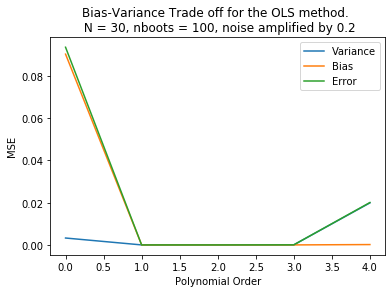
\includegraphics[width=65mm]{figure7.png}
}
\subfloat[Ridge]{
  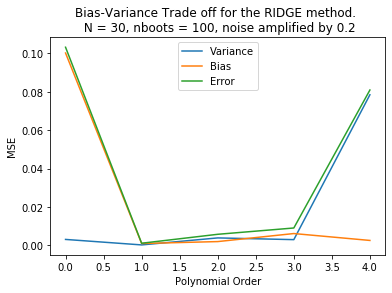
\includegraphics[width=65mm]{figure8.png}
}
\newline
\subfloat[Lasso]{
  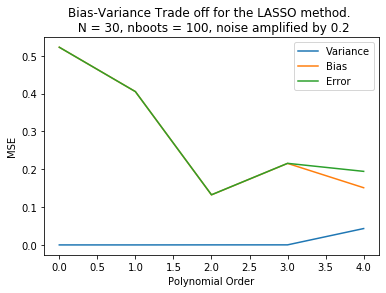
\includegraphics[width=65mm]{figure9.png}
}
\caption{Here are three bias-variance trade-off plots for our three different statistical methods using the bootstrap method for resampling.\newline
Based on what we're seeing here, we can assume that for fittings to polynomials of small orders, the OLS and Ridge methods are preferred, while the LASSO method looks to converge somewhere further along our x-axis.}
\end{figure}
\newpage
Now, let's take a look at the cross validation:
\begin{figure}[ht!]
\centering
\subfloat[OLS and LASSO]{
  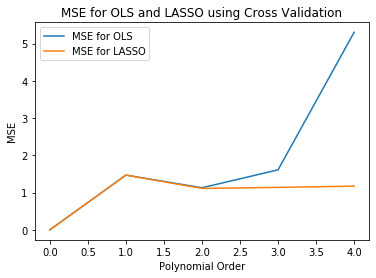
\includegraphics[width=65mm]{figure10.png}
}
\subfloat[Ridge]{
  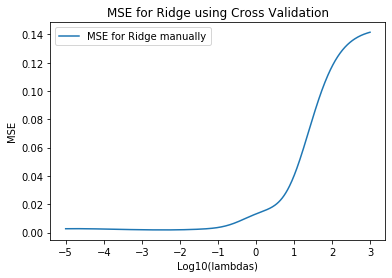
\includegraphics[width=65mm]{figure11.png}
}
\caption{Here we can see the MSE given a shrinkage parameter $\lambda$. OLS and LASSO are in their own plot using polynomial order because I couldn't get lambdas to work for those methods.}


\end{figure}
\newline
Let's now apply our Cross-Validation method onto our terrain data.
\begin{figure}[ht!]
\centering
\subfloat[CV-Result for Ridge Regression]{
  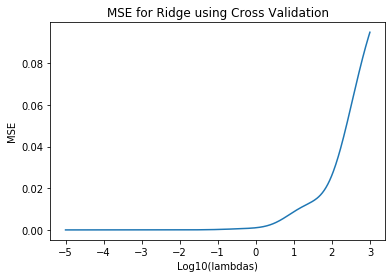
\includegraphics[width=65mm]{figure12.png}
}
\subfloat[The area of the map used]{
  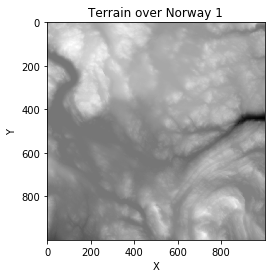
\includegraphics[width=65mm]{figure13.png}
}
\caption{Here we see the area of the map we're collecting data from and the MSE for a given lambda shrinkage parameter. \newline As explained in the caption for Figure [\ref{fig2}], I can't get it to work for OLS and LASSO, and as such we'll be using only Ridge.}
\end{figure}

\section{Discussion}
\subsection*{Discussing results}
For our Franke Function we can see that it's behaving as expected. We start off initially with a very underfit 3D plot, but as we approach the the ideal polynomial order we see that our statistical model more and more resembles the analytical solution. We also see that as we leave this 'Goldilocks Zone', for lack of a better term, we start having to deal with overfitting where the polynomial order becomes too high, and we get a very "wobbly" and exaggerated plot. This is especially prevalent in the $o = 27$ example, where the features of the analytical solution are greatly exaggerated. \newline
Further, lets look at the Bias-Variance Trade Off. While our results do mirror reality and look like "the real thing", I had some issues getting it to look nice. The Bias-Variance Trade-off plot is a pretty delicate process, and it can be hard to get nice results. As such, I don't think we should be too upset with what we got, but it does seem a bit "sharp". It feels as though variance should be a bit more "aggressive", but that might just be me not having much experience in this subject. That being said, ideally a Bias-Variance trade-off plot should look something like:
\begin{figure}[ht!]
    \centering
    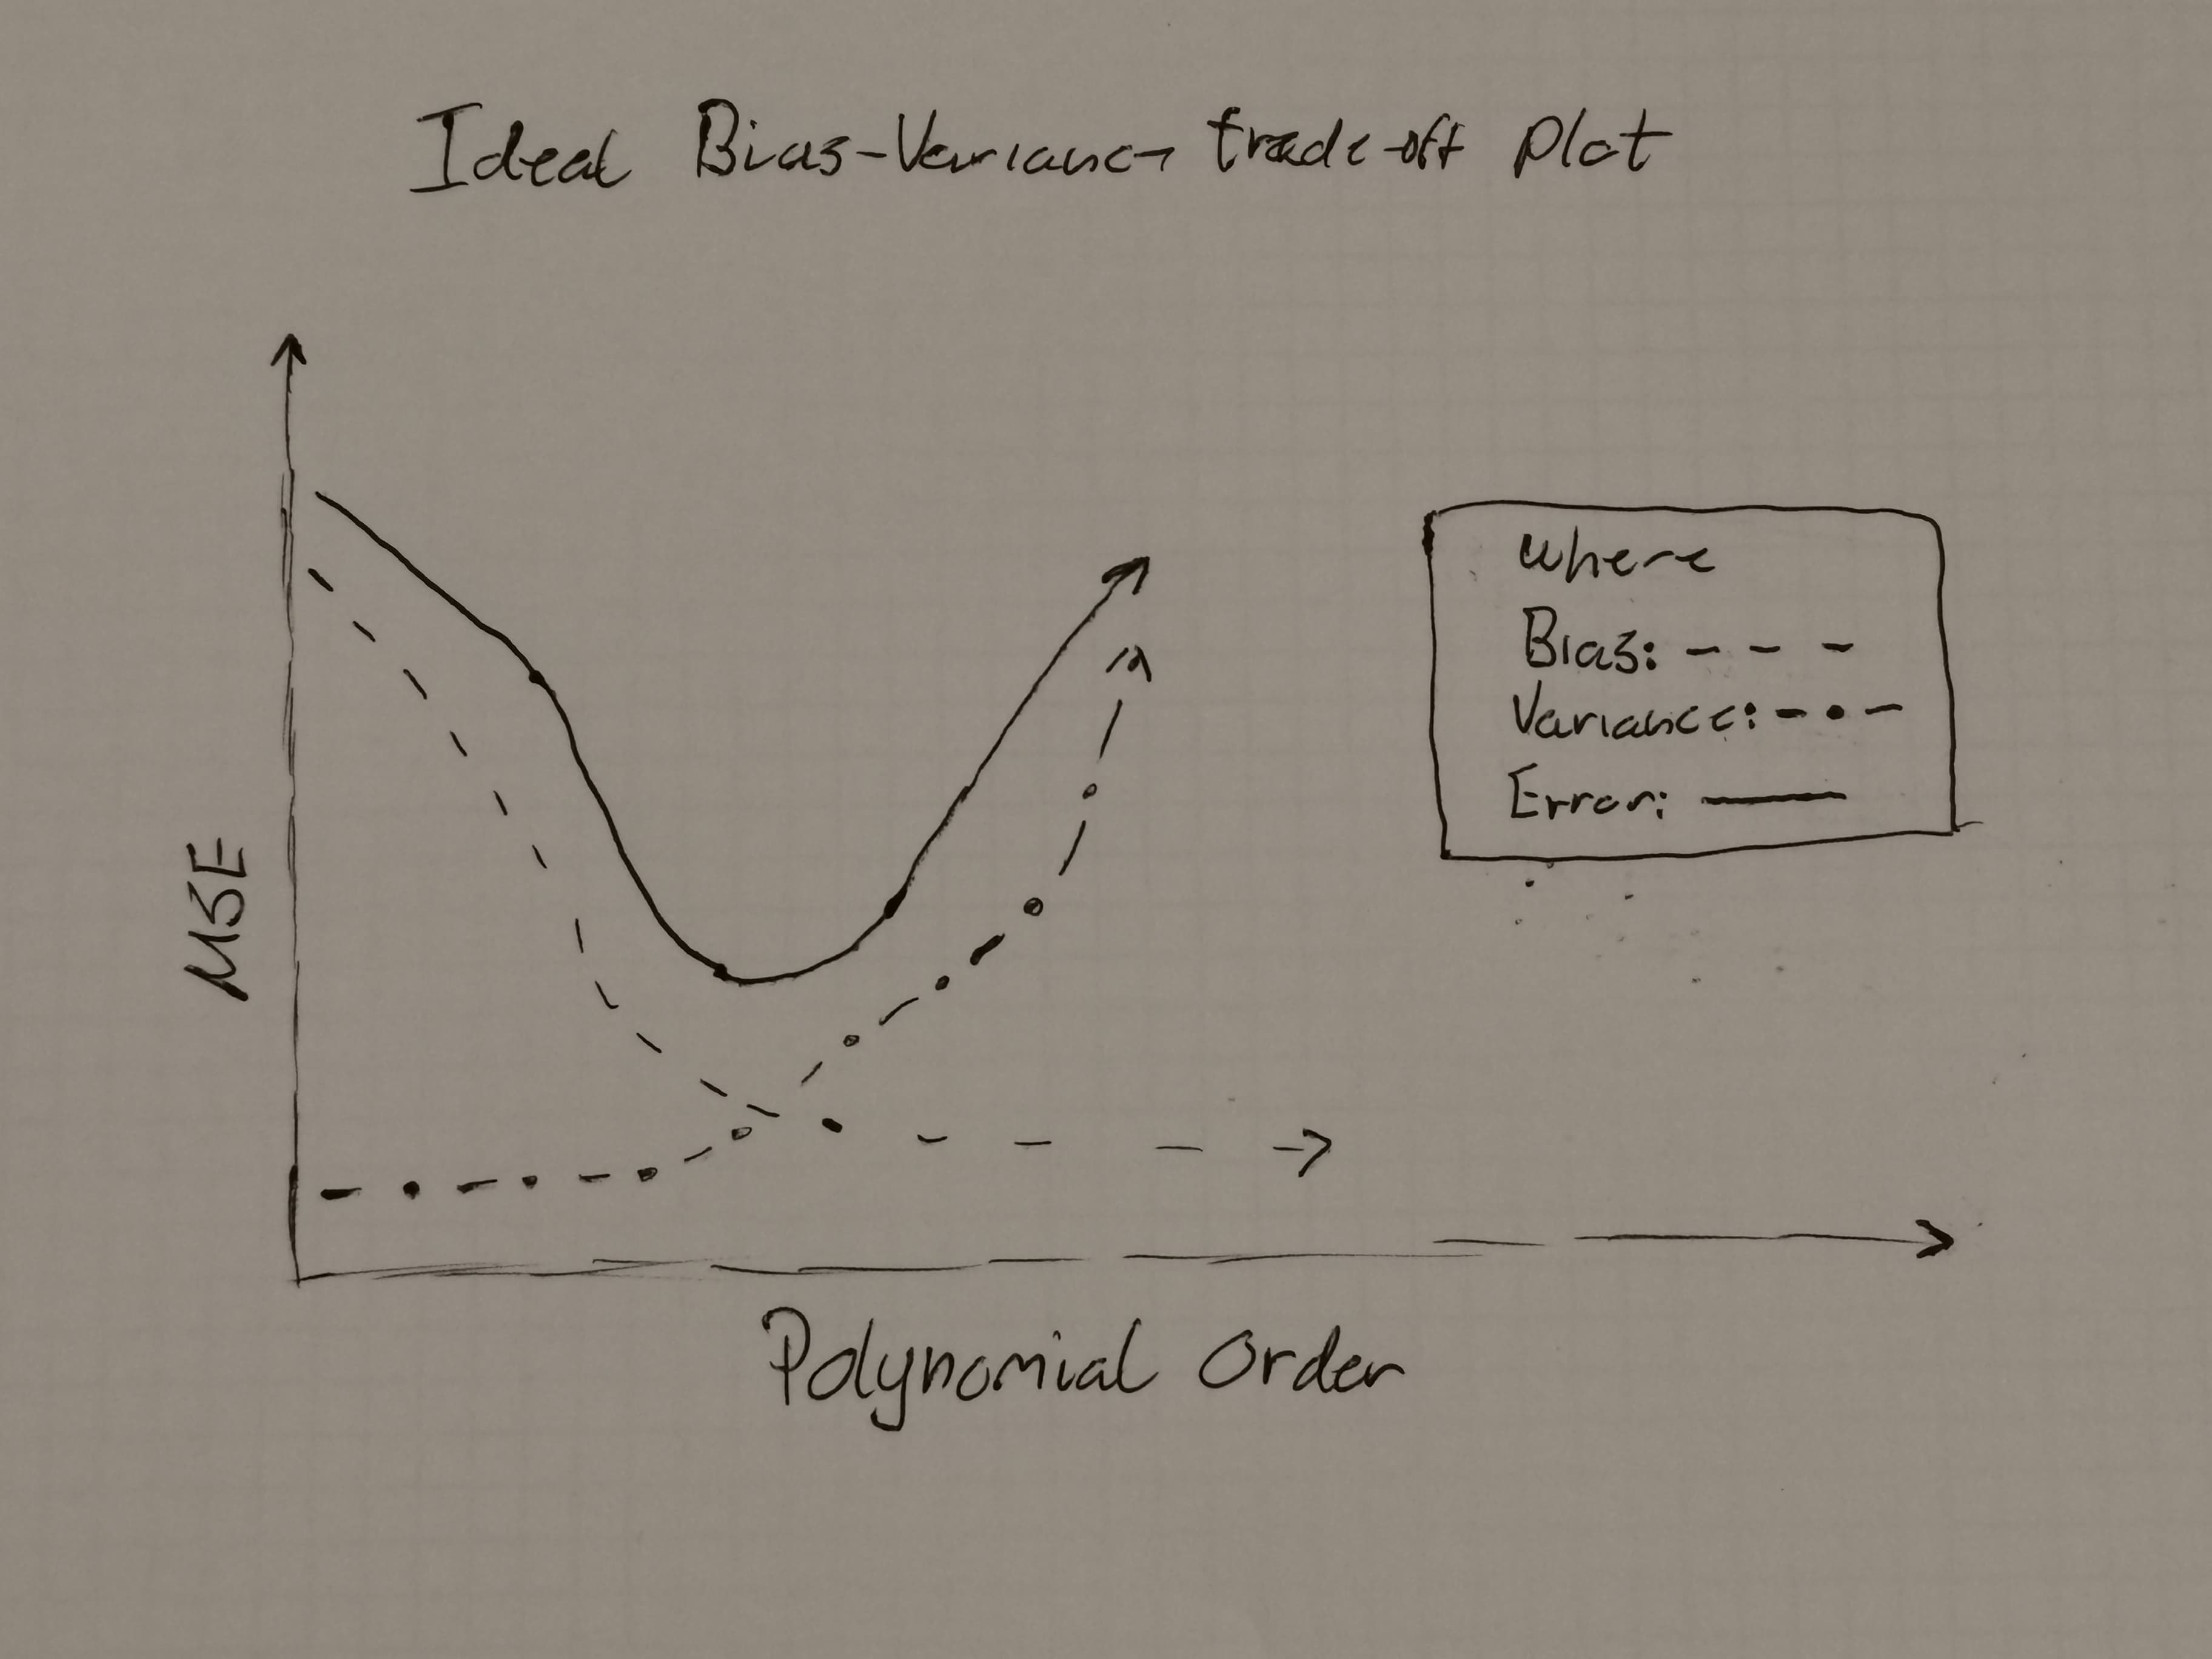
\includegraphics[scale=0.1]{figure14.jpg}
    \caption{An ideal Bias-Variance Trade-off plot \newline
    As we increase our polynomial order, the bias, or the deviation from our data points. However, if we increase too much, our variance begins to grow and takes over. Ideally you'd try to model using a polynomial order within the "Goldilocks Zone" where the Error is the lowest.}
    \label{fig3}
\end{figure}
\newpage
Next lets look at our Cross-Validation Plots. It's pretty hard for me to honestly and sincerely discuss these seeing as I'm pretty sure the leftmost plots are entirely wrong. However, for our rightmost plot we can see that for which shrinkage values our model gives us the least amount of error, in other words, our $lambda_{min}$.
We see much of the same for our terrain model's shrinkage plot. \newline
\subsection*{Code and reflection}
Like I said I had a lot of trouble getting my code to work. This is my first time ever working with statistics and any kind of machine learning/fitting outside of basic best-fit lines. Because of this I kind of realized a bit too late that I was a bit out of my depth in this subject, which probably comes off pretty clearly in this report.
\newline All in all for the latter part of the project I had some rather lackluster results, but I do hope it's not too bad, and at least passable.
\section{Conclusion}
In conclusion we've seen that fitting data to a model can be a tricky thing, and that different models have different strengths (at least in theory, not so much in execution in this case). Balancing our models can be a delicate process, where-in we need to carefully pick our variables like polynomial order, kfold, data points etc.
\bibliographystyle{unsrt}
\bibliography{citations.bib}
\section*{Appendix A - a few comments regarding the project}
\begin{itemize}
    \item I had a serious problem with pretty long run-times for fairly small polynomial orders (a big jump as $o = 7$). I was wondering if this was perhaps because I was using inefficient methods. I do recall hearing something about using pandas to handle our data sets. Could that improve my run-times (for next time)?
\end{itemize}
\end{document}
